\documentclass[a4paper,12pt]{article}
\usepackage{geometry}
\usepackage{fullpage} % Package to use full page
\usepackage{parskip} % Package to tweak paragraph skipping
\usepackage{amsmath}
\usepackage{hyperref}
\usepackage{amsmath,amsfonts,amsthm} % Math packages
\usepackage{graphicx}
\usepackage{listings}
\usepackage{color}
\usepackage{float}
\definecolor{codegreen}{rgb}{0,0.6,0}
\definecolor{codegray}{rgb}{0.5,0.5,0.5}
\definecolor{codepurple}{rgb}{0.58,0,0.82}
\definecolor{backcolour}{rgb}{0.95,0.95,0.92}
\definecolor{brown}{rgb}{0.59, 0.29, 0.0}
\definecolor{beaublue}{rgb}{0.74, 0.83, 0.9}
\definecolor{orange}{rgb}{1.0, 0.5, 0.0}
\definecolor{darkslategray}{rgb}{0.18, 0.31, 0.31}
\def\Xint#1{\mathchoice
	{\XXint\displaystyle\textstyle{#1}}%
	{\XXint\textstyle\scriptstyle{#1}}%
	{\XXint\scriptstyle\scriptscriptstyle{#1}}%
	{\XXint\scriptscriptstyle\scriptscriptstyle{#1}}%
	\!\int}
\def\XXint#1#2#3{{\setbox0=\hbox{$#1{#2#3}{\int}$}
		\vcenter{\hbox{$#2#3$}}\kern-.5\wd0}}
\def\dashint{\Xint-}

% Swap the definition of \abs* and \norm*, so that \abs
% and \norm resizes the size of the brackets, and the 
% starred version does not.
\makeatletter
\let\oldabs\abs
\def\abs{\@ifstar{\oldabs}{\oldabs*}}
%
\let\oldnorm\norm
\def\norm{\@ifstar{\oldnorm}{\oldnorm*}}
\makeatother
\lstdefinestyle{mystyle}{
	backgroundcolor=\color{white},   
	commentstyle=\color{codegreen},
	keywordstyle=\color{blue},
	identifierstyle=\color{brown},
	numberstyle=\tiny\color{codegray},
	stringstyle=\color{orange},
	basicstyle=\footnotesize,
	breakatwhitespace=false,         
	breaklines=true,                 
	captionpos=b,                    
	keepspaces=true,                 
	numbers=left,                    
	numbersep=5pt,                  
	showspaces=false,                
	showstringspaces=false,
	showtabs=false,                  
	tabsize=2
}
\lstset{style=mystyle}

\title{\normalsize AMATH 535: Homework Problem 5.2}
\author{\normalsize Jithin D. George, No. 1622555}
% matrix environment
\newenvironment{mat}{\left[ \begin{array}{ccccccccccccc}}{\end{array}\right]}
\newcommand\bcm{\begin{mat}}
	\newcommand\ecm{\end{mat}}

\begin{document}

\maketitle
	
{\bf 	} 



{\bf Solution:	}

\begin{enumerate}
	\item
Here, the logistic growth term is plotted in red while the functional response is in green.
\begin{figure}[H] 
	\centering
	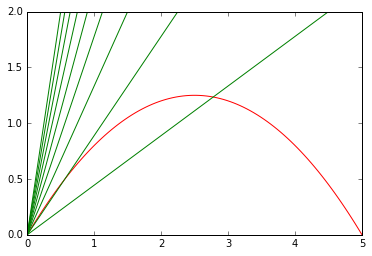
\includegraphics[width=8cm]{som2}
	\caption{Functional response 1}
\end{figure}
For the first functional response, the number of equilibria are 1 or 2.
\begin{figure}[H] 
	\centering
	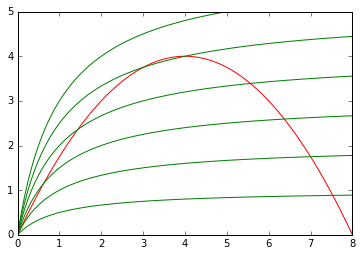
\includegraphics[width=8cm]{som1}
	\caption{Functional response 2}
\end{figure}
For the second functional response, the number of equilibria are 1,2 or 3.




\begin{figure}[H] 
	\centering
	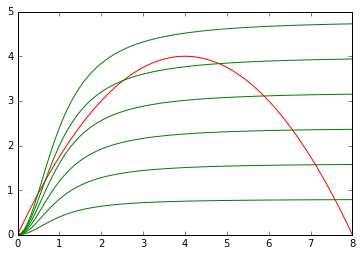
\includegraphics[width=8cm]{som3}
	\caption{Functional response 3}
\end{figure}
For the third functional response, the number of equilibria are 2,3 or 4.


\item
Here are the bifurcation diagrams.

\vspace{3cm}

\begin{figure}[H] 
	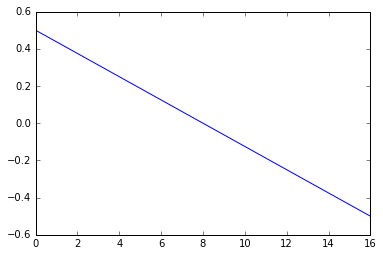
\includegraphics[width=8cm]{som11}
	\caption{Functional response 1}
\end{figure}

\vspace{3cm}
\begin{figure}[H] 

	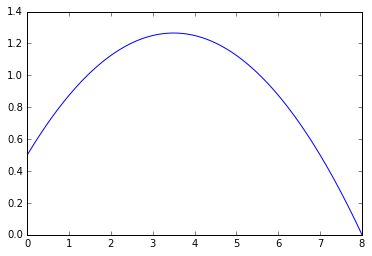
\includegraphics[width=8cm]{som12}
	\caption{Functional response 2}
\end{figure}

\vspace{3cm}

\begin{figure}[H] 
	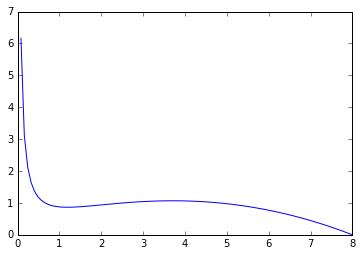
\includegraphics[width=8cm]{som13}
	\caption{Functional response 3}
\end{figure}


\end{enumerate}
\end{document}